\documentclass{ds-report} 
\usepackage{babel}[english]
\usepackage{graphicx}
\usepackage{url}

\assignment{Project} % Set to `Remote communication` or `Project`.
\authorOne{Martijn Leplae} % Name of first team partner.
\studentnumberOne{r0737706} % Student number of first team partner.
\authorTwo{Andreas Hinderyckx} % Name of second team partner.
\studentnumberTwo{r0760777}  % Student number of second team partner.

\begin{document}
	\maketitle

	\paragraph{Question 1}
	The component diagram can be found as figure \ref{fig:component}. We show every component in a `component'-box, along with relevant class objects/concepts in yellow boxes. The half open circles and full circle arrows indicate required and offered interfaces respectively.
	
	The front-end exists of the computer of the customer, which can be seen on the left hand side of the diagram. The back end consists of the Google cloud Component platform on one hand, and the Theatre servers on the other hand.
	
	The front-end makes use of the interface offered by the Spring boot server. Within the back-end, the firebase authentication server offers an interface both to the frond-end and the Spring boot server endpoints to decouple the authentication of users. Within the Google App engine we also make use of a Pub/Sub server whose job is to delegate JWT messages from the Model to the theatre ICompany servers, when it comes to confirming quotes. Other HTTP-requests are sent directly form the Model class to the ICompany servers. This Pub/Sub server makes use of the endpoint made available in the Pub/Sub-controller's interface.
	\paragraph{Question 2} 
	We've made use of the Spring boot API to be able to simply create an endpoint te receive the messages of our Google Pub/Sub implementation. For this scenario, we could simply add the \texttt{@RestController} annotation and provide the code which corresponds to this endpoint. The specific behaviour of receiving POST-requests can then be added by providing the method with an \texttt{@PostMapping} annotation.
	
	The addition of Pub Sub API hides the complexity of implementing a subscription service for clients to subscribe to certain topics. 
	
	\paragraph{Question 3} 
	In the method that confirms requested quotes (i.e. transforms them into bookings), we've made use of the Pub/Sub API to make the process of a client requesting a booking and the server confirming it asynchronous. 
	
	The steps that occur in the indirect communication are:
	 \begin{itemize}
	 	\item The channel of the project, \texttt{Topic} and \texttt{PubSubMessages} instances are created,
	 	\item Create a \texttt{Publisher} which publishes \texttt{PubsubMessage}s for a given \texttt{Topic} on the channel created above.
	 	\item The message containing the quotes to be booked and required attributes are serialized and sent over the channel by the publisher as a \texttt{PubsubMessage}.
	 	\item Next, on the subscriber side, at our custom endpoint, the messages are received and unmarshalled and parsed into its original form.
	 	\item Finally, a PUT request is performed for each quote to confirm its corresponding booking on the theater ICompany server.
	 \end{itemize}
 
 	\paragraph{Question 4}
 	Taking our endpoint created in function of the Pub/Sub mechanism as background worker, the marshalled form of the list of quotes to be booked is passed, along with other required parameters to perform the PUT-request: the API key and the name of the customer who makes the bookings. 
 	
 	If the server were physically separate machine, it wouldn't be able to make a reference to the object of the client. Therefore, it makes sense to marshall a copy of the quotes and send this to the server side such that it has its own local copy to work with.
	
	\paragraph{Question 5}
	For our small scale application, the indirect communication (Pub/Sub) only introduces some extra delay when confirming a booking due to the asynchronous nature of Pub/Sub. This implementation becomes advantageous, however, when scaling the application to a larger scenario. Then a large amount of applications or clients can all make use of the same Pub/Sub server, subscribers can easily filter out the messages they want to receive out of a common channel these are sent over.
	
	\paragraph{Question 6}
	As mentioned above, for small scale scenarios such as that of our application, the client only perceives increased delay due to the asynchrony introduced by Pub/Sub.
	
	\paragraph{Question 7}
	It should not be possible to perform a double booking with our implementation. Our approach is as follows: when a client wants to make a series of bookings, these are stored in a list and sequentially placed in a PUT request to try to obtain the corresponding ticket. As soon as one of these quotes can't be booked, the entire list of tickets conform to the requested bookings is deleted with a corresponding DELETE-request. As we are allowed to assume that these DELETE-requests are fully reliable and the ICompany is assumed to be reliable as well --- as mentioned in the assignment --- this approach ensures that only the client who books his ticket first can obtain it: any other client trying to obtain the same ticket afterwards, will receive an error in the PUT request and thus will have its requested tickets removed from the server.
	
	\paragraph{Question 8} 
	Suppose there are multiple groups of people where each group has a different list of permissions. If we were to store a list of people who are allowed to perform a certain task and were to do this for each task, it would quickly become cumbersome to check whether a certain user is allowed to perform a certain task. Analogously, if a new user is to be added, one would need to manually add this user to each list of each task this user is allowed to perform.
	
	With role based access control, this gets simplified to checking the permissions of a user's role, or assigning the appropriate role to a new user respectively.
	
	\paragraph{Question 9}
	The encoding the authentication provider uses determines how we as implementer are to decode the incoming authentication cookies. A change of authentication provider therefore implies refactoring this decoding process. In our case, if another provider were not to use the JWT web tokens, our implementation of the manager verification would need to be re-implemented, too.
	
	A new authentication provider must at least provide the ability to add roles to users, in order to make use of the role based access control mechanism. 
	
	\paragraph{Question 10}
	Each time the unreliable theater ICompany reports a failure in its response, we wait for a set time period before re-sending the same request again. We repeat this procedure until a successful response of the ICompany is received. The faultier the server becomes, the higher the delay the client perceives. Thus to set the delay between each request
	one must make a trade-off between making sure enough time has passed for the faultiness to have disappeared, and making sure that the client doesn't perceive a delay which is too lengthy. 
	
	Another possibility is only try to re-send the request a fixed set of times. This way the delay can't build up indefinitely, but at the same time the client isn't guaranteed to be served the requested page when the faulty server does load. 
	
		\paragraph{Question 11} 
	NoSQL affects both elements as follows:
	\begin{enumerate}
		\item \textbf{Scalability}:
		\begin{itemize}
			\item NoSQL is easily scalable: instead of needing to upgrade the hardware (i.e. CPU) one can simply add extra servers to distribute the load. 
			\item New data can be incorporated into the database more easily, instead of needing to redesign the entire schema of an SQL-database.
			\item 
		\end{itemize}
		\item \textbf{Availability}:
		\begin{itemize}
			\item  The data is then duplicated, which increases redundancy to mitigate the effect of crashes or failures of certain servers.
			\item It can be spread geographically, thus making it easy to make available to lots of places in the world.
			\item Data can be stored `as is', that is: it needs not to be transformed in order to be put into the database, but can rather be inserted using its original data types.
		\end{itemize}
	\end{enumerate}
	
	\paragraph{Question 12} 
	In our Firestore database we have set up three collections: "\texttt{LocalShows}", "\texttt{Bookings}", "\texttt{BestCustomers}". As primary keys, \texttt{UUID}s of the shows and bookings are used for the first two collections, and the customer's email address is used in the customers collection. \begin{itemize} 
		\item In \texttt{BestCustomers} we keep track of the number of tickets per customer. This facilitates efficient querying for the \texttt{getBestCustomer} method, as we do not need to scan every customer's list of bookings.
		\item The collection \texttt{Bookings} is used to store the bookings. 
		\item \texttt{LocalShows} holds the local shows. However, we opted to set up two subcollections here: \texttt{Seats} and \texttt{showTimes}. We do this for the following reasons:
		\begin{enumerate}
			\item It makes the querying of an individual Seat way easier and faster E.g when querying a specific seat of a show, no other data needs to be send over the net, all the querying happens in Firestore. This prevents the combinatorial explosion of looping over all possible seat-time combinations.
			
			\item The showtimes could be derived from the seats. However, in that case we would need to download all the seats and do a lot of querying ourselves. For this reason, having a separate collection for the Showtimes is worth the small amount of data duplication in return for efficient querying.
		\end{enumerate}
	\end{itemize}
	%Subcollections are used to further facilitate querying, as this minimises the required parsing and increases structure in the data model.
	
	\paragraph{Question 13} 
	NoSQL offers a much more limited querying interface. It is not possible to link data from different collections together using the NoSQL querying interface. To resolve this, a new collection must be made containing these queried elements. In the case of SQL, one can use more intricate queries without needing to make modifications to the data model.
	
	\paragraph{Question 14} 
	In the case of all-or-nothing semantics with the remote companies, the DELETE-request made to undo a failed booking might fail too, whereas using a transaction guarantees that its effects can be rolled back when a failure occurs.
	
	With our previous implementation, we sequentially booked tickets one-by-one and rolled back one-by-one on failure. The transaction on the other hand first makes sure that all the seats can be booked (i.e. they are not already booked), and then makes all the bookings.
	
	\paragraph{Question 15} 
	The e-mail feedback is necessary as Pub-Sub handles the booking confirmation process, which means that this might incur some delay and that the web-interface won't be able to instantly show the confirmation of the booking to the user. Therefore, when a booking is made a confirmation e-mail is sent to the client to either confirm his booking or to report that his booking didn't succeed. Based upon this information the client may re-submit his booking in case of failure or may be reassured of the success of his booking in case of success.
	
	\paragraph{Question 16} 
	In case of peak usage of the website --- e.g. when there would be a lot of interest in a certain show at a specific time --- we could prepare for this by reducing the \texttt{max\_pending\_latency} and \texttt{min\_pending\_latency} to make sure that enough instances will be available to accommodate for the peak usage.
	We only changed the \texttt{min\_instances} to a small positive value to minimise the loading times for the first visitor (as there is then no extra waiting time incurred for starting up the first instances). The other default values seemed to be fine since we don't expect lots of traffic. In essence there will always be a trade-off between making the scaling more responsive on one hand, and limiting costs on the other hand.
	
	\paragraph{Question 17} 
	\begin{enumerate}
		\item The advantages of running an application as a web service are:
		\begin{itemize}
			\item Reduced hardware needs: the application can be ran from any device with an internet connection, rather the being limited to devices with hardware sufficiently powerful to run the application,
			\item Increased fault-tolerance: local applications only have a single copy of the stored information, whereas a web service can leverage on the advantages of a distributed setting where the information is duplicated across multiple geographically different locations. This leads to overall increased availability,
			\item Independence of the hardware the application is run on: native applications need to be ported to every supported hardware and operating system configuration, whereas an application running as a server is independent of these factors, 
			\item The software is automatically up-to-date, which means the users don't need to do updates themselves. (e.g. there are still people using old software that doesn't have recent security patches for example).
		\end{itemize}
		\item Deploying the project in the cloud has the advantages of leveraging on Google's large server infrastructure, which allows for seamless scaling in combination with the automatic allocation of extra instances when needed. This also eliminates the hassle that comes with your own server infrastructure. Besides, the cost of setting up a remote-accessible server is much lower with Google's pay-as-you-go cost model, in comparison to the cost and time involved in acquiring your own hardware and setting this up.
	\end{enumerate}
	
	\paragraph{Question 18} 
	Pitfalls of migrating a local project to the cloud include:
	\begin{itemize}
		\item Correctly implementing security,
		\item Learning to work with and link together the broad spectrum of APIs used in a cloud environment,
		\item You become dependent of the ecosystem your cloud provider offers: it may not be easy to change this without modifying a lot of code and/or configuration details, as well as missing out on certain features that are offered by one provider but aren't by another provider.
	\end{itemize}
	Restrictions of Google Cloud include;
	\begin{itemize}
		\item Google Cloud allows for third party token verification when using Firestore. This increases flexibility and customisation, at the risk of improper security implementations,
		\item Google Cloud lots of different APIs which must be correctly tied together in a project,
		\item Debugging becomes more time consuming, as the logs are only visible after a noticeable delay, and the source code itself can no longer be stepped through to debug potential issues. Deploying takes around a minute, so when you want to see the effect of a (potentially small) change on the cloud deployment, you need to wait for a while.
	\end{itemize}
	
	\paragraph{Question 19} 
	A lot of the code we wrote is specific to make use of the Google Cloud APIs, which means that this all of this code must be rewritten when migrating to a different cloud provider. For example, storing data in the Firestore database required code to specifically connect to this database, create specific data structures (\texttt{collection}s and \texttt{document}s), retrieve this data in a specified manner, etc. This also holds for authentication, pub-sub, etc. So we would need to find alternatives for these on the other provider.
	Additionally, certain providers may offer a different set of features or APIs which won't be offered by different providers, potentially requiring you to re-design or re-develop certain functionalities.
	
	\paragraph{Question 20} 
	We simulated multiple concurrent visitors of the website by opening 8 different browser windows and using the page (approximately) concurrently.  Assuming that the users visit the website uniformly across the 24 hour time-span of one day, this results in a total of two instances being spawned which gives us an estimate of two users that can be handled per instance.
	We simulated a use case of an average user who books several seats at different shows and recorded the number of read and write operations made in Firestore. This turns out to be approximately $280$ read, $5$ write and $0$ delete operations. Extrapolating this to $1000$ daily users, we get roughly $280 000$ read, $5000$ write and $0$ delete operations (as the user has no possibility of deleting his bookings). The current total amount of data used is 0.02GB, which is mainly dominated by the storage to store the local shows. The bookings themselves only require a limited amount of storage, thus we estimate that scaling this up to 1000 daily users will amount up to 0.5GB. Debugging our Pub Sub code shows that this same use case creates a message of size approximately $650$ bytes.This gives us a total estimate of 0.065 MB of Pub Sub messages per issued per day. Inputting all this information in the Google Cloud Pricing Calculator (\url{https://cloud.google.com/products/calculator/#id=1781479a-9372-4643-922f-09bbfefa4b2e}), gives us a total monthly cost estimate of 871.43 dollars per month.
	
	Increasing the daily number of users per day to one million, we analogously retrieve a monthly cost estimate of 923,345 dollars per month (based on our rough estimates). As the major part of this monthly cost comes from Google App Engine, this cost can be reduced by reducing the minimum and maximum number of instances, increasing pending latencies and reducing the maximum number of concurrent requests in the \texttt{app.yaml} configuration file. At this scale of number of daily users, however, it would be more cost effective to use regular server APIs of Google rather than App Engine which don't incur costs for automatic scaling, etc. Possibly, setting up an own server infrastructure might be more cost effective in the long run, too, at this scale.
	
	\clearpage
	
	% You can include diagrams here.
	
	\begin{figure}
		\begin{center}
			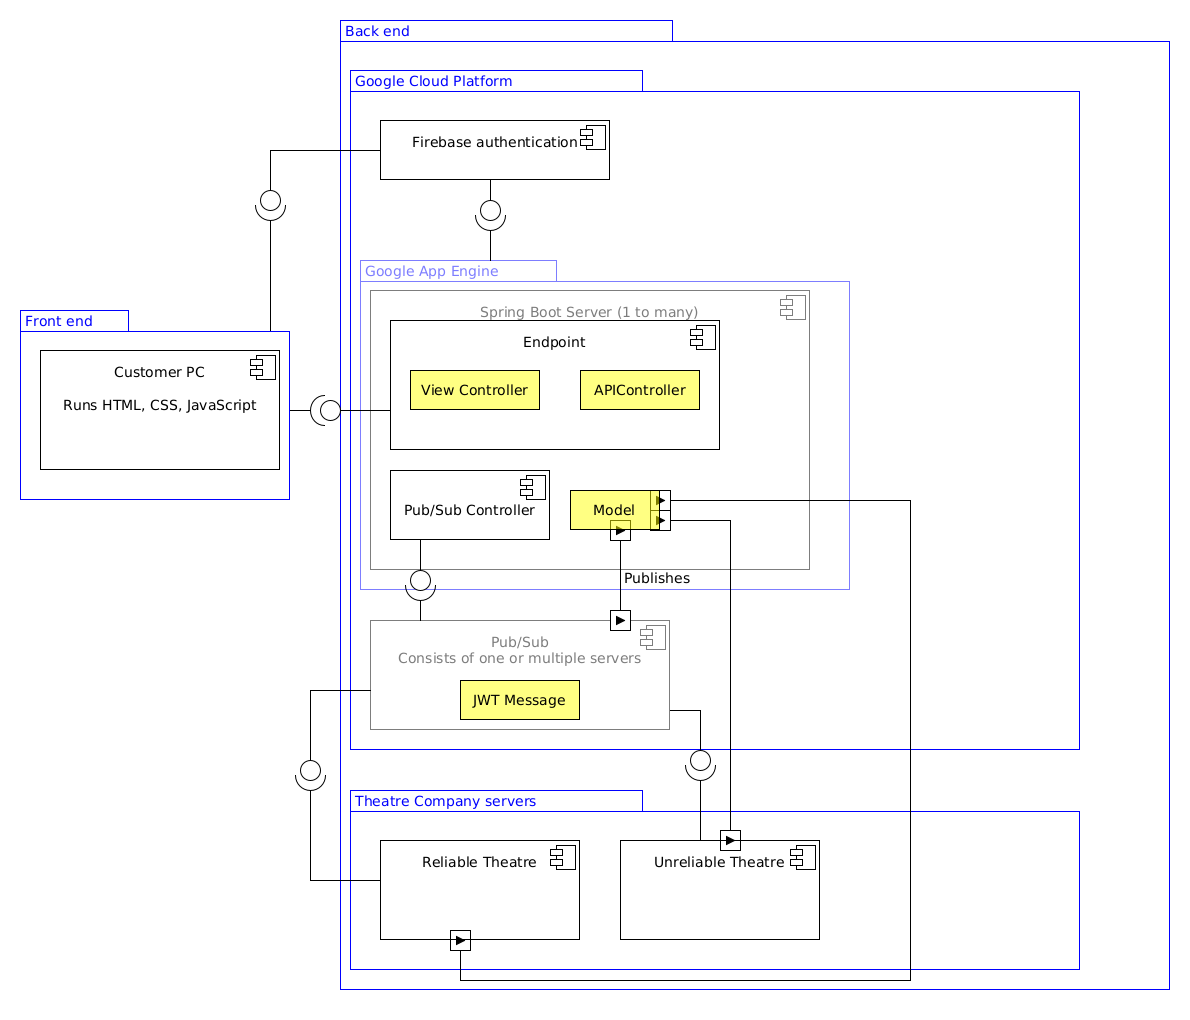
\includegraphics[width=\linewidth]{./diagrams/ComponentDiagram}
		\end{center}
	\caption{Component diagram of part I of the project.}
	\label{fig:component}
	\end{figure}

	
\end{document}